\documentclass[12pt]{article}
 \usepackage[margin=1in]{geometry} 
\usepackage{amsmath,amsthm,amssymb,amsfonts}
\usepackage{graphicx} 
\usepackage{tabularx} 


\begin{document}
 
 
\title{Analysis and Classification of Crimes in Chicago}
\author{Ye Zhou}
\maketitle
 
\section{Definition}
\subsection{Project Overview}
Historically, Chicago saw a major rise in violent crime starting in the later 1960s [1]. More recently, the crime situation in Chicago is getting even worse. Last year, Chicago has experienced a recent spike in homicides of 762 people, an increase of 58 percent over 2015 [2]. Compared with other largest cities in United States, Chicago has a significantly higher murder rate than New York or Los Angeles [3]. There is no denying the fact that crimes have become a severe social concern for Chicago as prosperous communities in the long term. 
Here, we are interested to analyze the Chicago crime data through visualization tools in python, and make predictions for the category of crimes given time and location, using machine learning algorithms.
\subsection{Problem Statement}
This project is aimed to predict the Chicago crime type based on time and position information. The raw data from Chicago Data Portal is preprocessed to the features (year, month, weekday, hour, location description, community, latitude and longitude) and target variable (crime type), and then split into train, test and validation dataset (6:2:2). After an exploration in the visualization of the crime data, we will apply logistic regression (benchmark model) and xgboost algorithm with finely tuned parameters on the train and test dataset. The performance of two algorithms will be evaluated with log loss function and accuracy and finally reported on the validation dataset.

\subsection{Metrics} 
This project use the log loss function and accuracy, from sklearn.metrics package, to train the model and evaluate the performance.
\section{Analysis}
\subsection{Data Exploration}
The data is imported from the Chicago Data Portal website [4], which is a collection of city data related not only to crimes, but also to education, transportation, health, and so on.
The dataset has 21 columns:
\begin{itemize}
\item ID - Unique identifier for the record.
\item Case Number - The Chicago Police Department RD Number (Records Division Number), which is unique to the incident.
\item Date - Date when the incident occurred. this is sometimes a best estimate.
\item Block - The partially redacted address where the incident occurred, placing it on the same block as the actual address.
\item IUCR - The Illinois Unifrom Crime Reporting code. This is directly linked to the Primary Type and Description.
\item Primary Type - The primary description of the IUCR code.
\item Description - The secondary description of the IUCR code, a subcategory of the primary description.
\item Location Description - Description of the location where the incident occurred.
\item Arrest - Indicates whether an arrest was made.
\item Domestic - Indicates whether the incident was domestic-related as defined by the Illinois Domestic Violence Act.
\item Beat - Indicates the beat where the incident occurred. A beat is the smallest police geographic area – each beat has a dedicated police beat car. Three to five beats make up a police sector, and three sectors make up a police district. The Chicago Police Department has 22 police districts.
\item District - Indicates the police district where the incident occurred.
\item Ward - The ward (City Council district) where the incident occurred.
\item Community Area - Indicates the community area where the incident occurred. Chicago has 77 community areas.
\item FBI Code - Indicates the crime classification as outlined in the FBIs National Incident-Based Reporting System (NIBRS).
\item X Coordinate - The x coordinate of the location where the incident occurred in State Plane Illinois East NAD 1983 projection. This location is shifted from the actual location for partial redaction but falls on the same block.
\item Y Coordinate - The y coordinate of the location where the incident occurred in State Plane Illinois East NAD 1983 projection. This location is shifted from the actual location for partial redaction but falls on the same block.
\item Year - Year the incident occurred.
\item Updated On - Date and time the record was last updated.
\item Latitude - The latitude of the location where the incident occurred. This location is shifted from the actual location for partial redaction but falls on the same block.
\item Longitude - The longitude of the location where the incident occurred. This location is shifted from the actual location for partial redaction but falls on the same block.
\item Location - The location where the incident occurred in a format that allows for creation of maps and other geographic operations on this data portal. This location is shifted from the actual location for partial redaction but falls on the same block.
\end{itemize}

    From the variables above, we plan to extract the year, month, weekday (from Monday to Sunday) and hour features from the column ‘Date’. And the positional information is described by a combination of ‘Location description’, ‘Beat’, ‘District’, ‘Ward’, ‘Community Area’, ‘Latitude’ and ‘Longitude’.  The information of ‘IUCR’ and ‘FBI Code’ are excluded, because these they contain the crime classification information.
    
    The ‘Primary Type’ of crimes is the target variable for prediction in our models, which has 33 categories in the 2016 crime data. To make the model more robust and efficient, here, we transform the ‘Primary Type’ to major crime types (theft, battery, criminal damage, assault, deceptive practice, burglary, narcotics, robbery, motor vehicle theft), and severe crime type (homicide). Figure shows the occurrence of different crimes in Chicago from 2015 to 2016.
\begin{figure}[h]
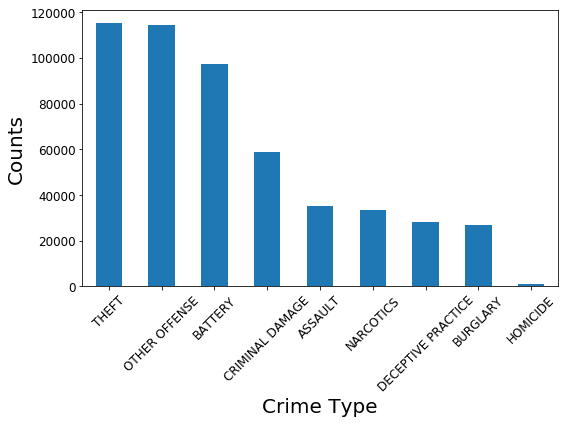
\includegraphics[scale=0.5]{figure/total_crime.png}
\centering
\caption{The occurrence of crimes in Chicago from 2015 to 2016}
\end{figure}
  
  
The whole dataset will be split into train, test set (6, 4) for the model development.
\subsection{Exploratory Visualization}
\subsection{Algorithms and Techniques}
\subsection{Benchmark Model}
\section{Methodology}
\subsection{Data Preprocessing}
\subsection{Implementation}
\subsection{Refinement}

 
\section{Results}
\subsection{Model Evaluation}
\subsection{Justification}


 
\section{Conclusion}
\subsection{Free Form Visualization}
\subsection{Reflection}
\subsection{Improvement}

\end{document}
